This section discusses information regarding an initial time plan for the project, tollgates to be respected, activities and what resources that's available.

\subsection{Time and resource plan}
As previously mentioned HeartByte have 160 hours per employee as a budget in this project. This is a time limit that has to be respected. Apart from human resources, we do also have knowledge resources, that are to be further developed if needed. HeartByte is able to consult other companies within the same industry in order to get a certain knowledge or program-module available.\vspace{5mm}

Regarding time plan, the project is divided into five different externally decided iterations, please see the figure below for information regarding dates. Since it has been decided to work in a SCRUM-manner in the project, the iterations later in time hasn't been populated with detailed tasks. This is to be done later in the project as progress is made. 
\begin{center}
    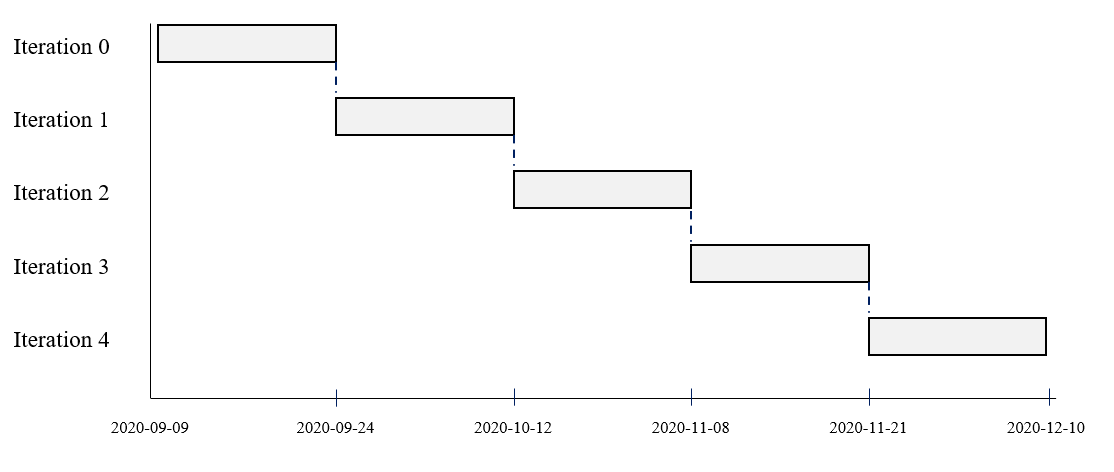
\includegraphics[width=\linewidth]{all_iterations}
\end{center}
   
\subsubsection{Iteration 0}
Iteration 0, also called for the pre-study phase, is a time where HeartByte is to get to know the customer and its needs.The main focus lies in understanding what value the system has to create and how this could be done. As a result of this, HeartByte is to pursue workshops where ideas regarding how this expected value creation can take place and how the product should be created.
\begin{center}
    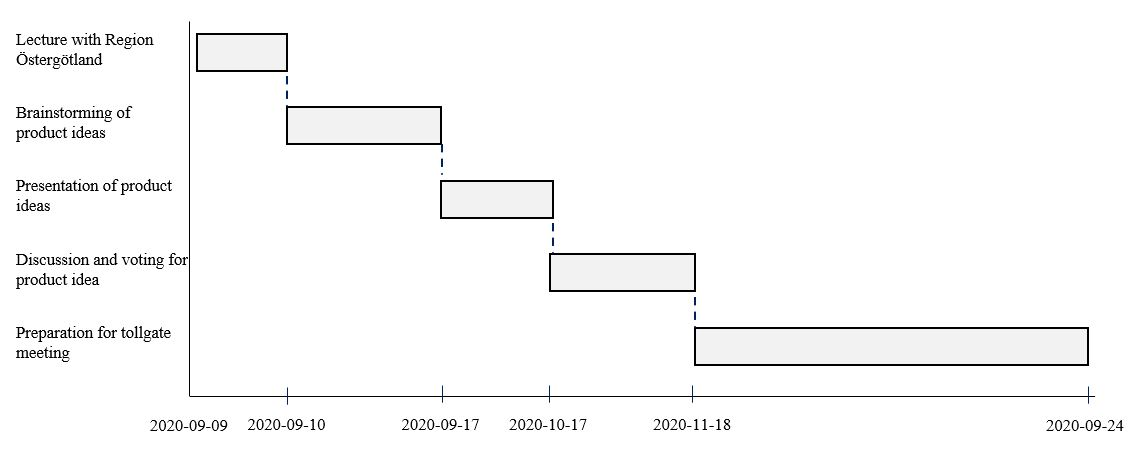
\includegraphics[width=\linewidth]{iteration_0}
\end{center}

The pre-study phase ends with a tollgate meeting where HeartByte is to present the results of the studies that has been made. The customer, Region Östergötland are to decide if they support further development of the idea brought to the Table by HeartByte.

\subsubsection{Iteration 1}
When the customer has accepted the proposed product, HeartByte is entering iteration 1. In this iteration, the main focus is to create a list of requirements and get it accepted by the customer and to educate the employees with the correct knowledge according to their positions. Also the idea of testing is to be given attention, starting off with lo-fi tests pursued with a lo-fi prototype. The idea of this process is to get comments from intended users if the planned product is functional or not, or if there are any major aspects that has to be redone.

\begin{center}
    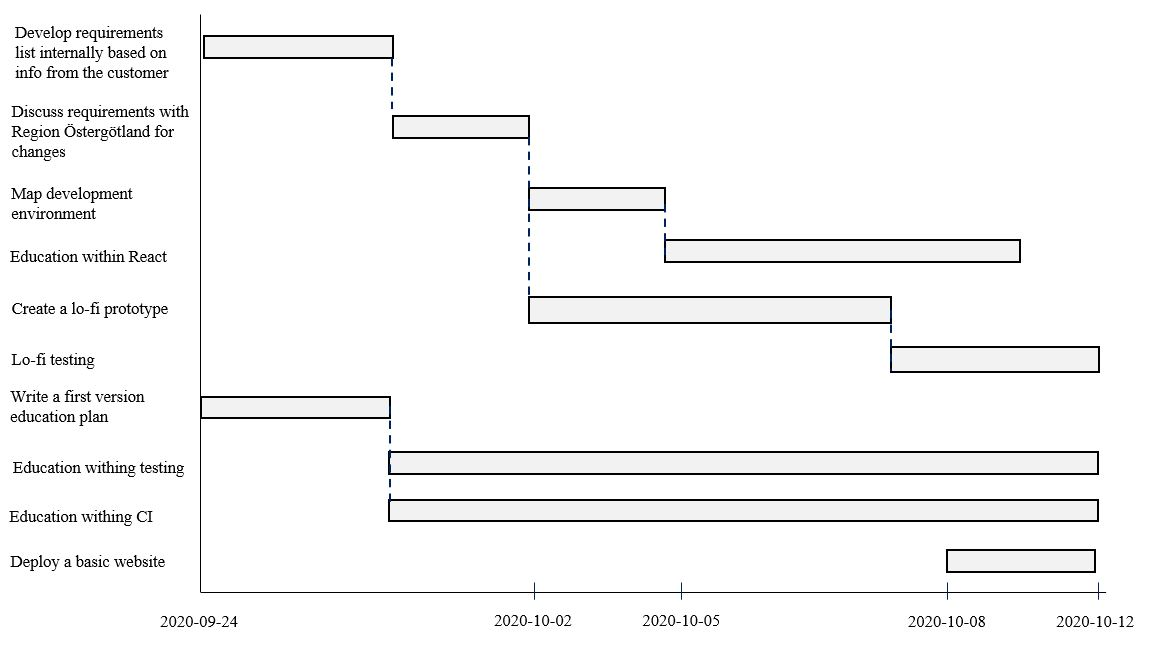
\includegraphics[width=\linewidth]{iteration_1}
\end{center}
The idea is that HeartByte should be able to start coding and develop at the end of this iteration. In order to be able to do so, the initial list of requirements has to be accepted by the customer and the developers need to have applicable knowledge within decided coding language. A CI environment should be set up in order to enable continuous integration and development. 

\subsubsection{Iteration 2}
Iteration 2 holds more or less exactly 2 weeks of effective working time since it is to be interrupted by the exam period in the middle of it. The main focus for this iteration is to get a basic product / web page to be functional and accessible. This puts a constraint on our development environment; before HeartByte is able to have a functional web site online, a working CI pipeline is required. 
\begin{center}
    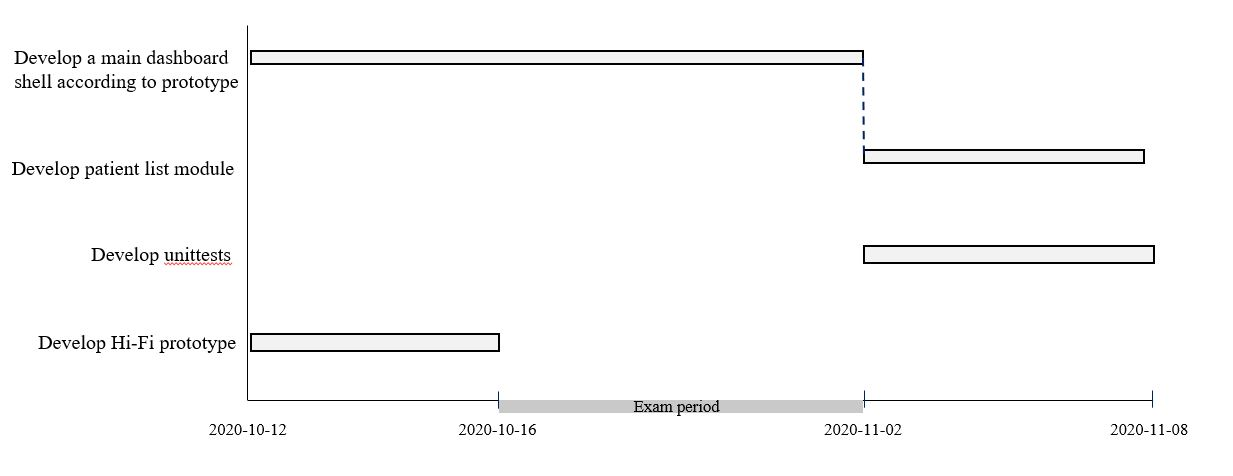
\includegraphics[width=\linewidth]{iteration_2}
\end{center}
The tasks that populates the Gantt-schema above are subject for change in the upcoming period of time since the mapping of the development phase is to be done. To increase the efficiency of the development, a hi-fi prototype is to be developed as well, serving as a blueprint for the developers. This also enable more proper testing with intended end-users. 

\subsubsection{Iteration 3}
Iteration 3 stretches from 2020-11-08 until 2020-11-21. In this iteration the main plan is to develop the features with lower priority since the features with higher priority already has been developed at this time. When entering this iteration, the CI-pipeline should be populated with several unit tests as well as automated web tests developed with Selenium. Also, the system should be tested with our intended end-users. \vspace{5mm}
More information regarding this iteration is to be released further ahead in the project when more tasks can be mapped. Since the project is run in a SCRUM-manner, the list of tasks has to be flexible. 

\subsubsection{Iteration 4}
Iteration 4 stretches from 2020-11-21 until 2020-12-10. In this iteration, only one week is set aside for development with a planned coding stop 2020-11-28. The time after the code stop is planned to be used for documentation of the process but also preparation of the final delivery at VSSE that is to be held 2020-12-10. Testing and evaluation of the system is to be pursued as well. \vspace{5mm}
More information regarding this iteration is to be released further ahead in the project when more tasks can be mapped. Since the project is run in a SCRUM-manner, the list of tasks has to be flexible. 
\subsubsection{Planned tasks for development}
When the initial planning of the project was performed and done, the different development tasks and features could be planned when to be handled. The tasks didn't have that many links to each other and is for that reason not heavily dependent on each other. The tasks were divided into back-end and front-end specific tasks.
\begin{figure}[hbt!]
\centering
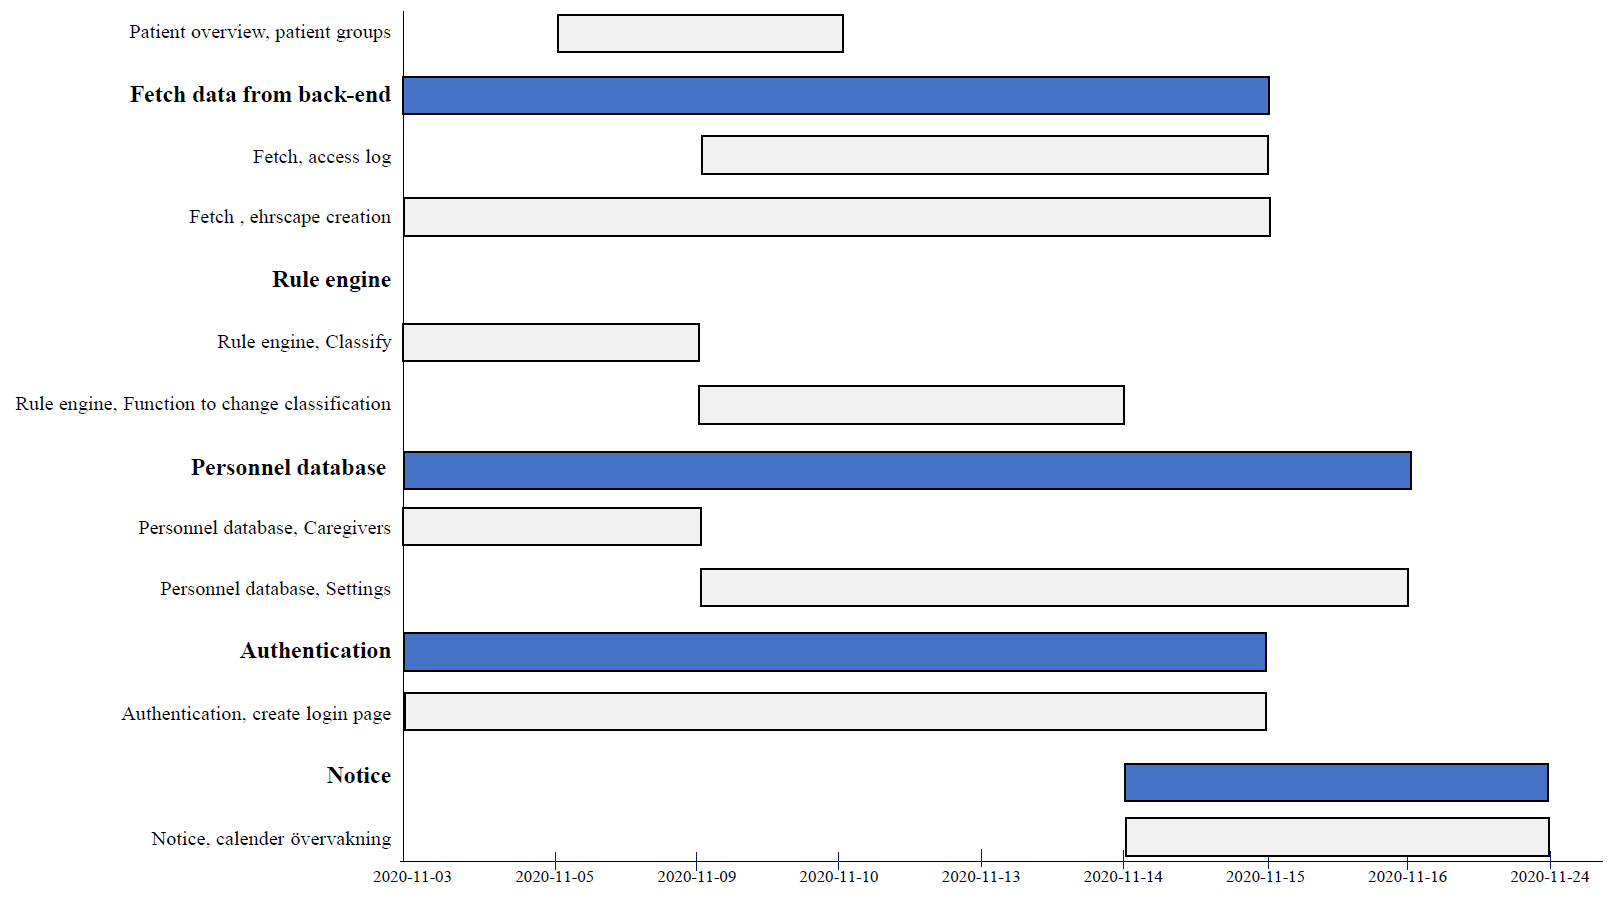
\includegraphics[width=\linewidth]{Pictures/DevTasksBackend.PNG}
\caption{Gantt-chart over planned tasks for the backend}
\label{fig:backend}
\end{figure}
\begin{figure}[hbt!]
\centering
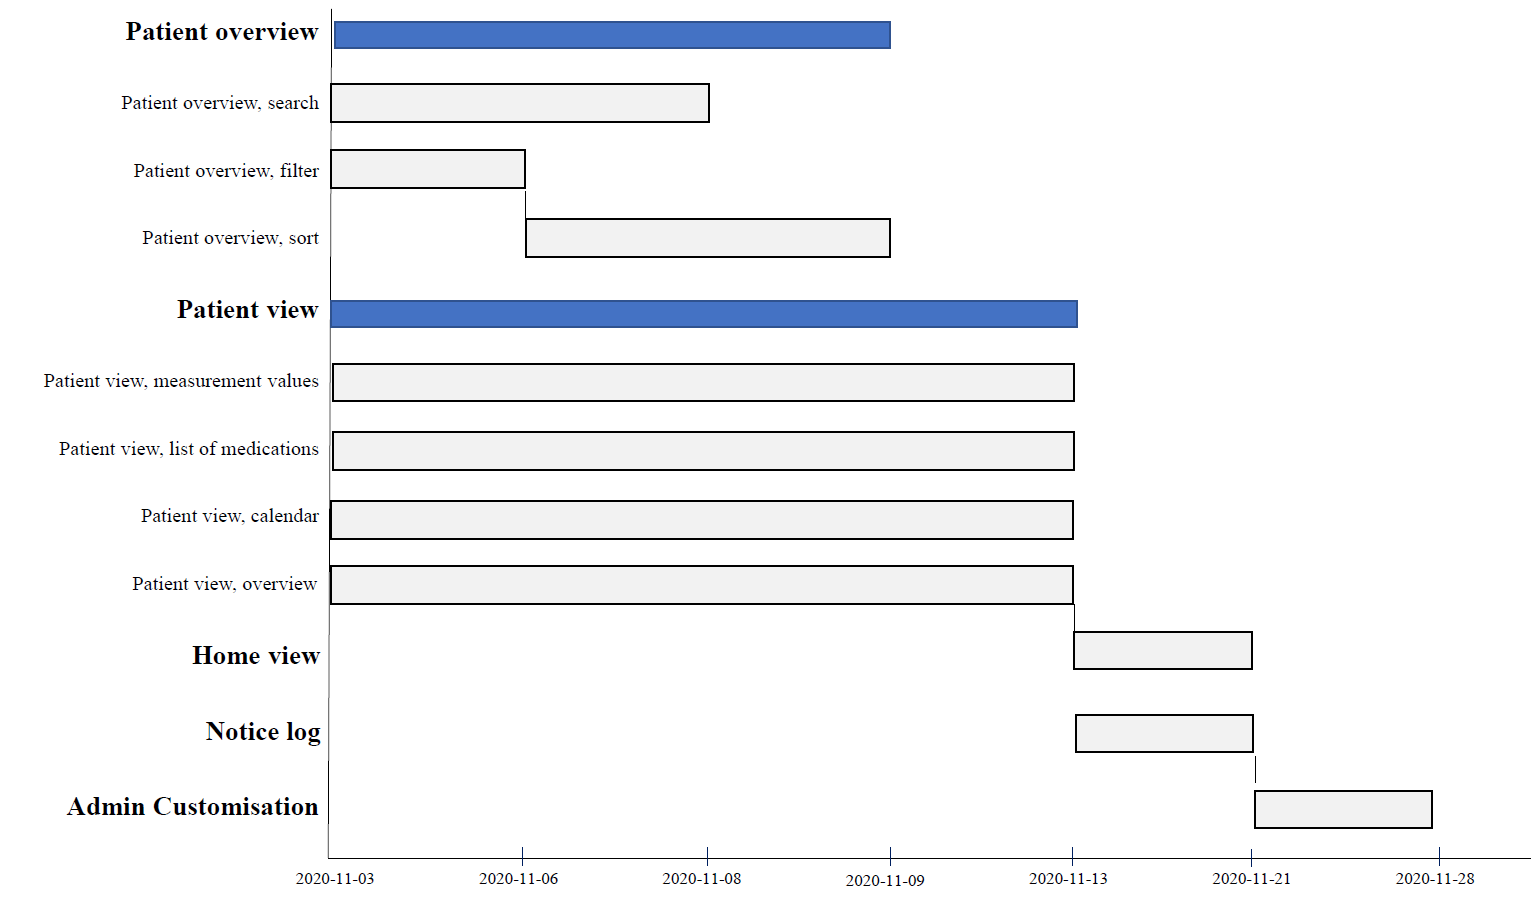
\includegraphics[width=\linewidth]{Pictures/DevTasksFrontend.PNG}
\caption{Gantt-chart over planned tasks for the frontend}
\label{fig:fronten}
\end{figure}

\newpage
\subsection{Tollgates}
A list of the currently defined tollgates is shown below. This list is to be further developed as the company agrees on certain dates for upcoming tollgates.
\begin{itemize}
    \item 2020-09-24 - The tollgate meeting with Region Östergötland\\ \\
    This meeting is about getting an approval from the customer that our idea for a solution creates the value needed for the customer. Before the meeting with the customer and external stakeholders were held, the entire organization for the project gathered to pursue a preparation meeting. During this meeting, the material provided from the management team to be presented on the tollgate meeting with the customer was discussed. The main purpose of this meeting is to give the entire project team a possibility to comment on the material being presented for our customer. Doing so, everyone can come up with changes in the material if they find that the management team is lacking in any circumstances when describing the pre-study phase. \\
    When this meeting was held, some minor comments were brought to the table by team members not being a part of the management group. The changes were implemented in the material to be presented for the customer before the main tollgate meeting. 
    \item 2020-10-12 - Basic CI-pipeline set up and an initial web application launched\\ \\
    The CI-pipeline has to be developed in order to enable a first version of the web application to be launched. This version of the web application is to be very simple. 
    \item 2020-10-14 - Development tasks \& responsibilities handed out \\ \\
    Since the product is to be developed in React, the entire product will be divided into different components. The initial idea is to divide these different components between smaller groups of developers in orders to create a more effective workflow.
    \item 2020-11-08 - A functional dashboard developed \\ \\
    The system has a dashboard where the user can press the buttons to enter a patient modal to retrieve information about the specific patient. 
    \item 2020-12-04 - Code stop for developing the product\\ \\
    Friday the 4th of December is the last day where it's allowed to push new code to the project. From this very date until delivery is time needed for last fixes of the delivery and deployment.
    \item 2020-12-10 - VSSE, the final presentation of the product\\ \\
    At this date the development of the product has to be fully terminated. The product has to be ready for delivery to the customer. 
\end{itemize}   

\begin{figure}[hbt!]
\centering
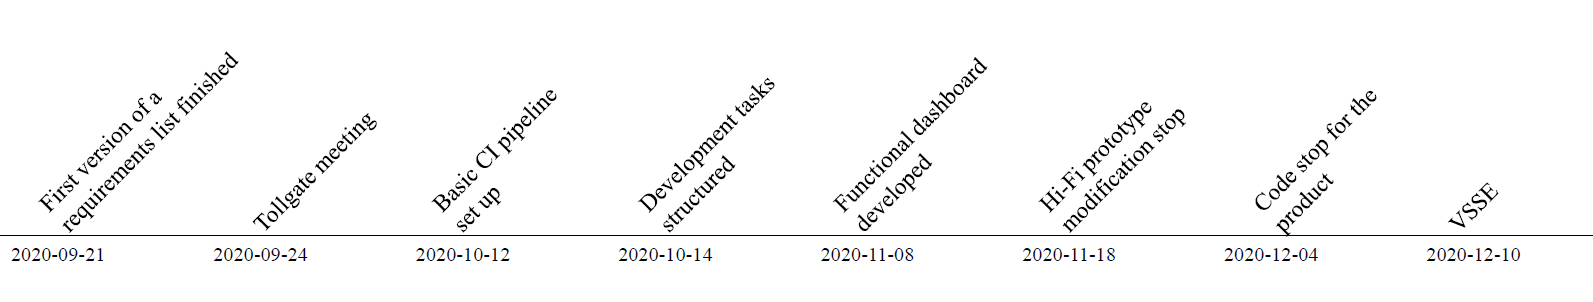
\includegraphics[width=\linewidth]{Pictures/timeline.PNG}
\caption{Timeline for what tollgates and deadlines the project is following}
\label{fig:timeline}
\end{figure}

\subsection{Deliverables}
Alongside the development of the software system and continuous delivery of the same, several supporting documents / artifacts are to be presented. These documents, like this project plan, is written to facilitate the development of a product in line with the customer requirements and available resources. Please find the a list of these documents and explanation of it's purpose below:
\begin{itemize}
    \item{\textbf{Project plan}} \\
    A document used to describe how the project is to be implemented as well for describing how testing and follow-up is to be done. 
    \item{\textbf{Software requirement specification, SRS}} \\
    Description of what requirements the customer has on the products that is to be delivered. The requirements are divided into functional and non-functional requirements and are also ranked regarding to it's importance for the system and customer. 
    \item{\textbf{Architecture notebook}} \\
    Description of how the architecture within the entire product / system is to be set up; how the database and front end is to be set up and how communication to external systems is implemented etcetera.  
    \item{\textbf{Test plan}} \\
    A document describing how the system is to be tested and how the documentation from the tests is to be maintained and stored. 
    \item{\textbf{Education plan}} \\
    How do we assure that the project organisation has the suitable knowledges for the different tasks? The education plan is set up to answer this question, meaning that the education plan is to be seen as a blueprint of how different knowledge needed within the project is to be acquired. 
    \item{\textbf{Software Quality Assurance, SQA}} \\
    Document describing how we are to assure a suitable quality on the product as well as for the processes implemented during the project. 
    \item{\textbf{Risk document}} \\
    Describing the risks with the project and how these risks are to be mitigated or avoided.
    \item{\textbf{Future Development}} \\
    Document to be developed in the end of the project. This document is to describe how the product is to be further developed after termination of the project. 
\end{itemize}
\subsection{Activities}
Below are a brief description of the main activities being implemented in the project and their intended outcome / meaning. 
\begin{itemize}
    \item{\textbf{Workshops}} \\
    Used to get the different team within the company together and to discuss future tasks and ideas. Workshops are to be planned several times during the project with different plans for each occasion. 
    \item{\textbf{Company meetings}} \\
    Meetings every Thursday where the entire company is brought together. Mostly used to discuss questions brought to the table by our external stakeholders or to discuss strategic matters for the project. 
    \item{\textbf{Mapping of requirements}} \\
    A process that is to be pursued together with the customer by our analyst team. The main reason for this task is to understand the many needs that our customer has and what requirements the product has to fulfill. 
    \item{\textbf{Development of Lo-Fi prototype}} \\
    A prototype firstly developed on paper without any functionalities. The main purpose for this prototype is to enable initial user testing as well as serve as a blueprint for the initial development / coding. 
    \item{\textbf{Writing of supporting documents}} \\
    The different documents mentioned above are written in order to enhance the performance for the entire company while working with this very project in different ways. 
    \item{\textbf{Lo-Fi testing}} \\
    Tests performed with the lo-fi prototype together with our intended end-users. The reason for this process being implemented is to get some initial comments on any eventual clear mistakes done in the first design phase. 
    \item{\textbf{Planning of education}} \\
    In order to be able to develop the product ordered by the customer, education has to be performed in a structured manner for the applicable sub-teams within the company. Therefore, writing an education plan is essential. 
    \item{\textbf{Mapping of requirements}} \\
    The team has to realize how the requirements stated by the customer is to be taken in consideration in the development process. 
    \item{\textbf{Development}} \\
    The actual coding / development of the product. This process is most definitely to be broken down into sub-tasks. 
    \item{\textbf{Testing}} \\
    Only performing lo-fi testing with our lo-fi prototype is not enough in order to ensure the customer that we are developing a product that will meet their requirements. Therefore, continuous unit- and web testing is required though out the development process. 

\end{itemize}






